\documentclass[12pt,a4paper]{article}
\usepackage{CJKutf8}
\usepackage{enumerate}
\usepackage{color}
\usepackage{graphicx}
\graphicspath{{./img/}}
\title{YokeEmulator 0.2.0.0 Manual}
\author{SxS\footnote{email:shinesong\_sxs@foxmail.com QQGroup:303579244}}
\begin{document}
\begin{CJK}{UTF8}{gbsn}
\maketitle

\section{Installation}
\begin{enumerate}[\textbf{Step} 1.]
\item Install vJoy 2.0.5.
\\*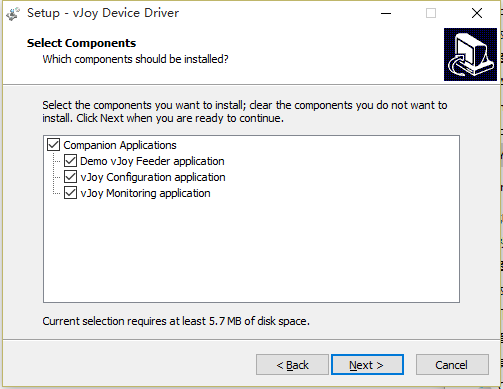
\includegraphics[width=4in]{install_vjoy.png}
\item Config vJoy use vJoyConf.
\\*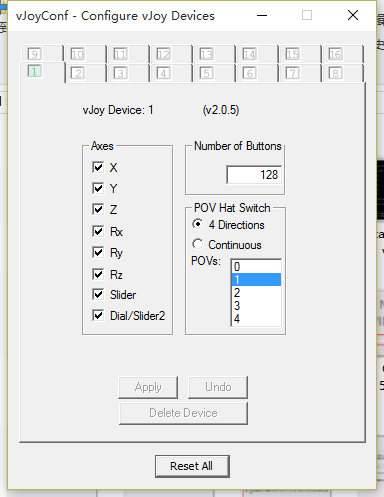
\includegraphics[width=4in]{install_config_vjoy.png}
\item Install .Net framework 4.5.2.
\item Test for YokeEmulatorServer,Like this
\\*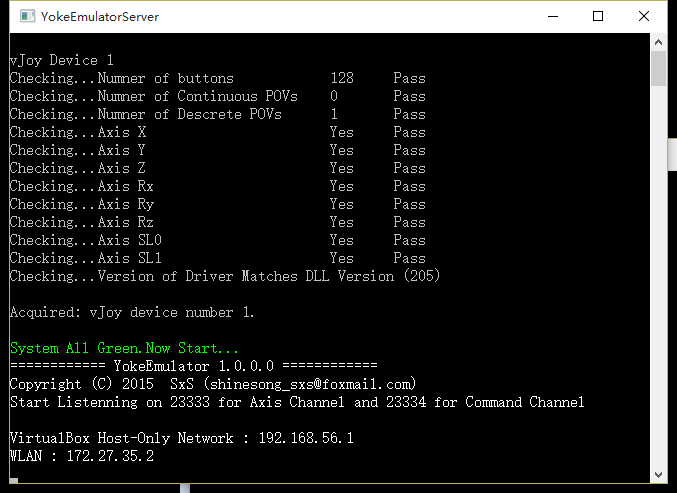
\includegraphics[width=4in]{install_finish_server.png}
\item Upload app to your unlocked WindowsPhone8.1 or upper.
\item Run App and set ip to your Computer in \textbf{Settings Page}.Make sure it's reachable.
\\*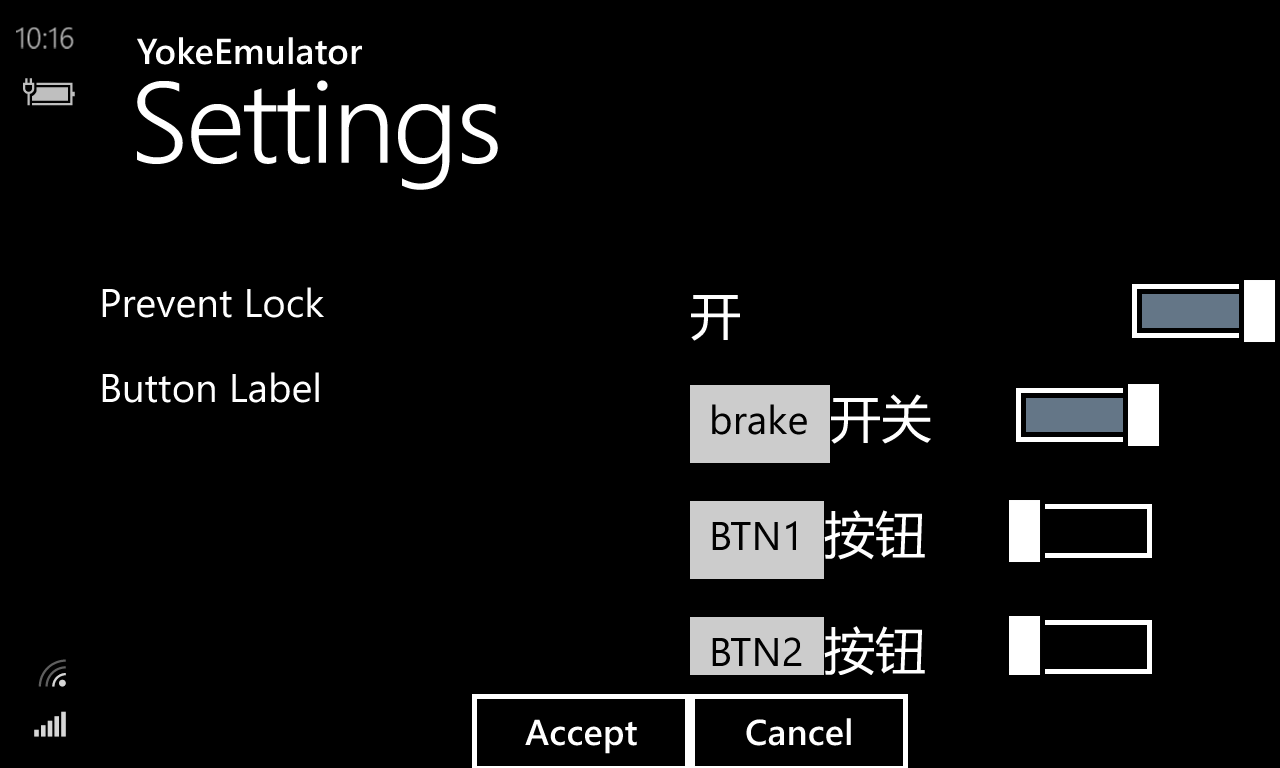
\includegraphics[width=4in]{install_app_settings.png}
\item Press \textbf{Connect} button on the left-top of screen,if success,it will turn to {\color{green}{DisConnect}}
\item Check vJoy Monitor to see if all program run well.
\\*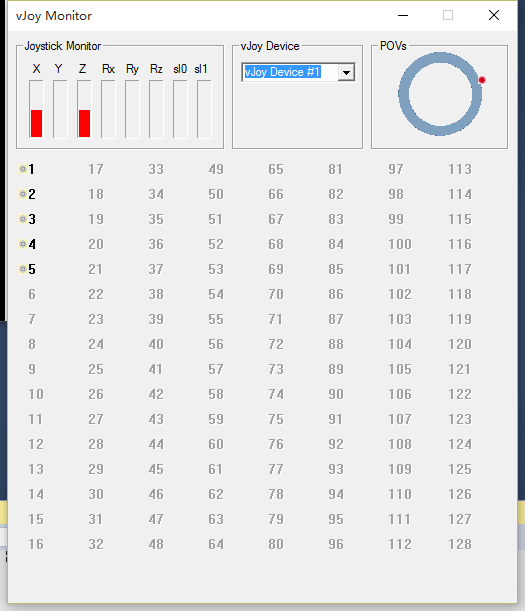
\includegraphics[width=4in]{install_test_yoke.png}
\item Enjoy it!
\\*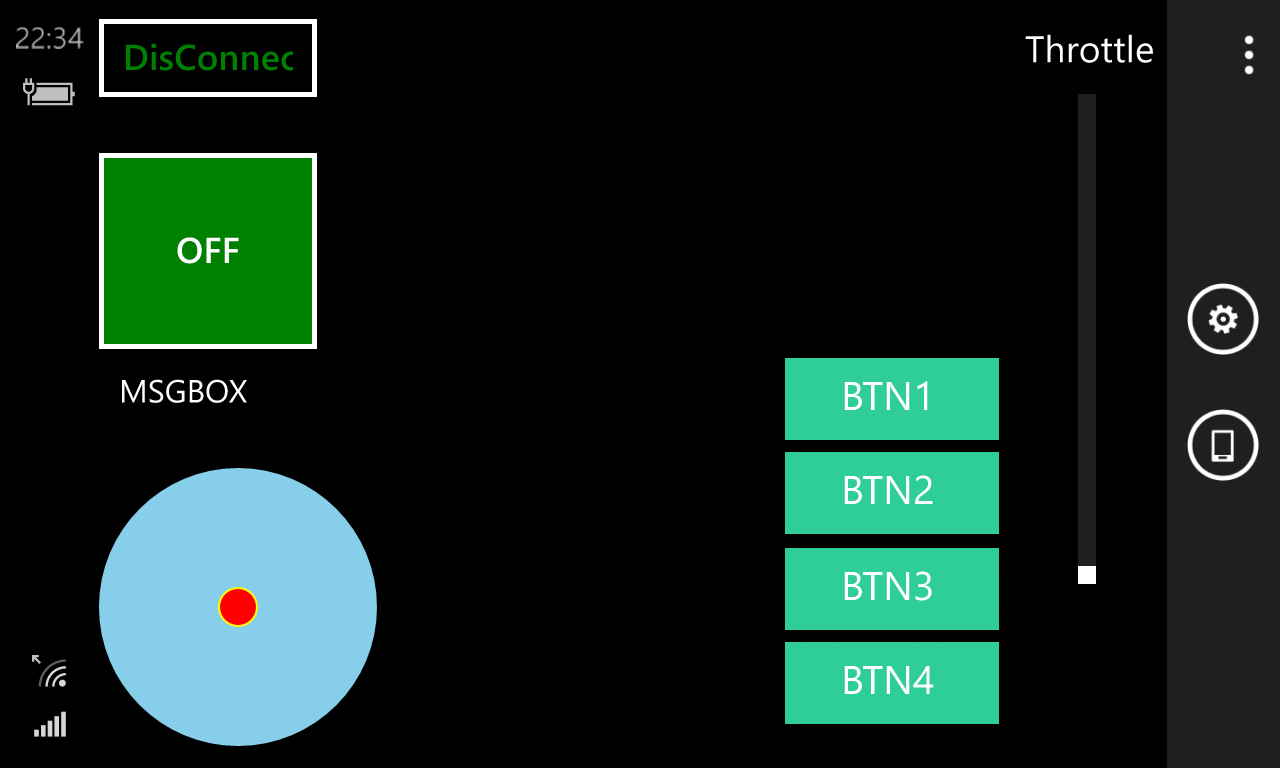
\includegraphics[width=4in]{install_finish_app.png}
\end{enumerate}
\section{Feature}
\subsection{0.2.0.0}
\begin{enumerate}
	\item Support for X Y Axis,Z for Rudder Axis,Slider Axis.Up to 128 buttons/toggle.Swithable Discrete 4 director Hat/Continual Hat;
	\item Customize Button/Toggle,Buttons Name;(See Settings page)
	\item Keep Screen unlock;
\end{enumerate}
\subsection{0.1.0.0}
\begin{enumerate}
	\item Support for X Y Axis,Slider Axis,4 buttons and Continual Hat;
\end{enumerate}
\section{TODO}
\emph{Exciting cool emurate track feature is developing.}
\end{CJK}
\end{document}
